%% LaTeX2e class for student theses
%% sections/content.tex
%% 
%% Karlsruhe Institute of Technology
%% Institute for Program Structures and Data Organization
%% Chair for Software Design and Quality (SDQ)
%%
%% Dr.-Ing. Erik Burger
%% burger@kit.edu
%%
%% Version 1.3.3, 2018-04-17

\chapter{Related Work}
\label{ch:related_work}

After having defined the objective and the research questions of this work, in this chapter we first introduce the basic concepts our approach builds upon.
We then discuss the state of the art in visualization approaches that deal with large document collections.

\section{Basic concepts}
\label{sec:basic_concepts}

This thesis unites two domains - information visualization and machine learning, more specifically \gls{nlp}.
This section introduces fundamental concepts from those two research fields that are not new, but serve as a foundation for our approach and a multitude of other works in visualization and machine learning.
Moreover, we introduce some terms related to the patent system, which are not a result of some particular existing research as such.
They are, however, together with the machine learning and visualization concepts mentioned above, the prerequisites necessary for a solid understanding of this work.

\subsection{Information visualization}
\label{subsec:information_visualization}

\subsubsection{Visual information seeking mantra}
\label{subsubsec:visual_information_seeking_mantra}

The visual information seeking mantra by Shneiderman \cite{Shneiderman1996} is a seminal concept that has contributed to the success of many powerful visualizations. It consists of three parts:
\begin{itemize}
\item overview first
\item zoom and filter
\item details on demand.
\end{itemize}
This guideline is crucial for providing optimal bandwidth of the presentation of information .

\textit{Overview first} means that in the beginning, a more abstract or zoomed out view of a document collection should be presented to the user. 
The goal at this point is to give a general impression without overwhelming the user.
Shneiderman \cite{Shneiderman1996} suggests complementing this view with a detail view. Together they yield a focus + context representation (see \autoref{subsubsec:focus_context}).

\textit{Zoom} allows users to satisfy their interest in some portion of the collection of data.
To support this, tools to control the zoom focus (the non-moving point the user zooms towards) and the zoom factor (the magnitude of the enlargement) are required.
Moreover, zooming should be smooth to preserve the sense of position and context.

\textit{Filter} essentially means applying dynamic queries to the items in the collection and hiding data points that are not in the result set. 
Filtering helps users to concentrate further on parts of the data they find interesting.
Shneiderman \cite{Shneiderman1996} argues that updating the display in less than 100 milliseconds is the goal.
Such reaction time is necessary to maintain the responsiveness of the system, so that users do not feel uncertain about the result of their action.

\textit{Details-on-demand} means that the detail view for a single data point should be shown after a request from the user such as clicking on the item. This constitutes the lowest abstraction level of working with a data collection.

\subsubsection{Focus + context}
\label{subsubsec:focus_context}

The basic idea with \textit{focus–plus–context}–visualizations is to enable viewers to see the object of primary interest presented in full detail while at the same time getting an overview–impression of all the \textit{surrounding} information — or \textit{context} — available.
Such visualizations are ``attention-warped displays''.
They attempt to use more of the display resource to correspond to the interest of the user's attention\cite{Card1999} - ``seeing the trees without missing the forest''.

\cite{Baudisch2002} provides an illustrative example of focus + context (see \autoref{fig:focus_context}).
\begin{figure}[!]
\centering
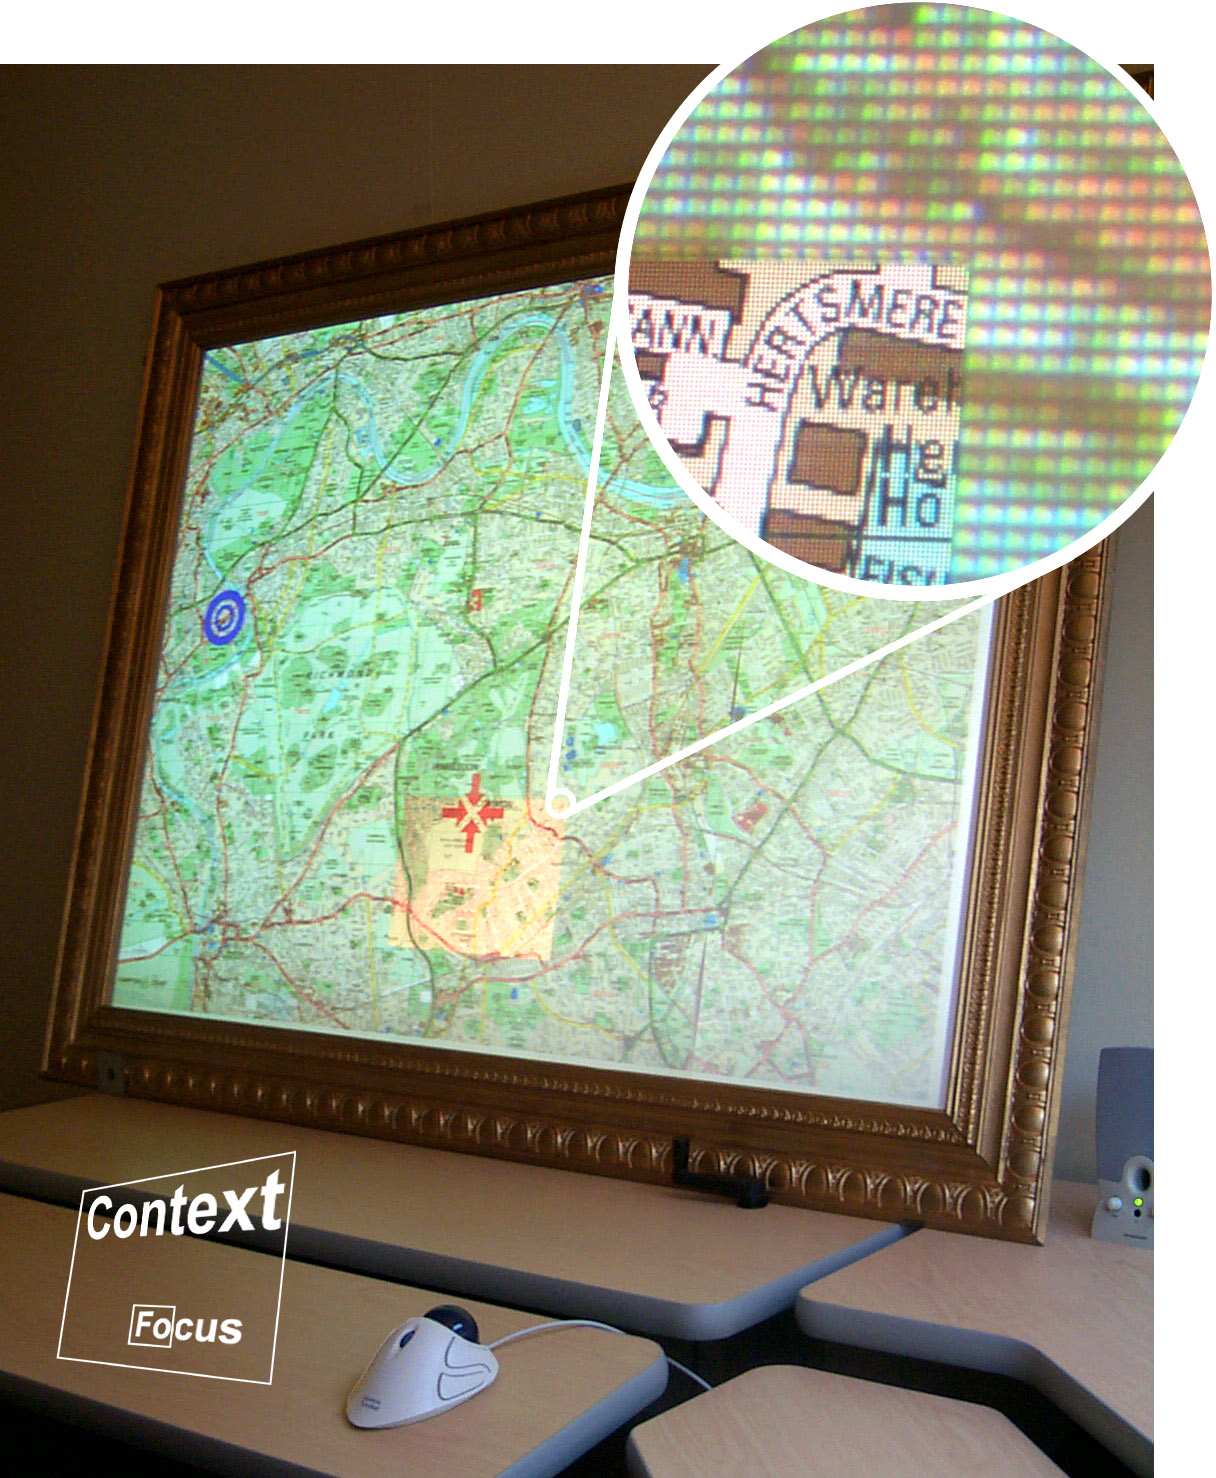
\includegraphics[width=\textwidth]{img/FullsizeMap}
\caption{A focus + context interface. 
The iconic illustration at the bottom left shows where the focus screen is located. 
The callout shows the different resolutions of focus and context area. Source: \cite{Baudisch2002}}
\label{fig:focus_context}
\end{figure}
They demonstrate a display that has an area with higher resolution nested inside a larger area with lower resolution.
A map is presented on the display, with its region of maximal interest (\textit{focus}) inside the area with higher resolution.
One can see that only this small region shows street names.

\todo{Define recognition over recall here?}

\subsubsection{Panning and zooming}
\label{subsubsec:panning_and_zooming}

``\textit{Panning} and \textit{zooming} refer to the actions of a movie camera that can scan sideways across a scene (panning) or move in for a closeup or back away to get a wider view (zooming)`` - \cite{hearst1999modern}.
This is an ubiquitous interaction form that creates a perception of space and movement in said space.
Is in most cases zooming is understood as physical zooming. For comparison with semantic zooming, see \autoref{subsubsec:semantic_zooming}.

\subsubsection{Semantic zooming}
\label{subsubsec:semantic_zooming}

A \textit{physical} zoom changes the size and visible details of objects. 
A \textit{semantic} zoom, on the other hand, changes the type and meaning of the information displayed by the object by using a semantic transition between detailed and general views of information \cite{Modjeska97}.

A thematically relevant example of semantic zooming is presented by Skupin \cite{Skupin2013}.
He automatically derives the thematic structure of a given domain.
As shown in \autoref{fig:som}, he visualized scientific publications from the field of biomedicine.

\begin{sidewaysfigure}[!]
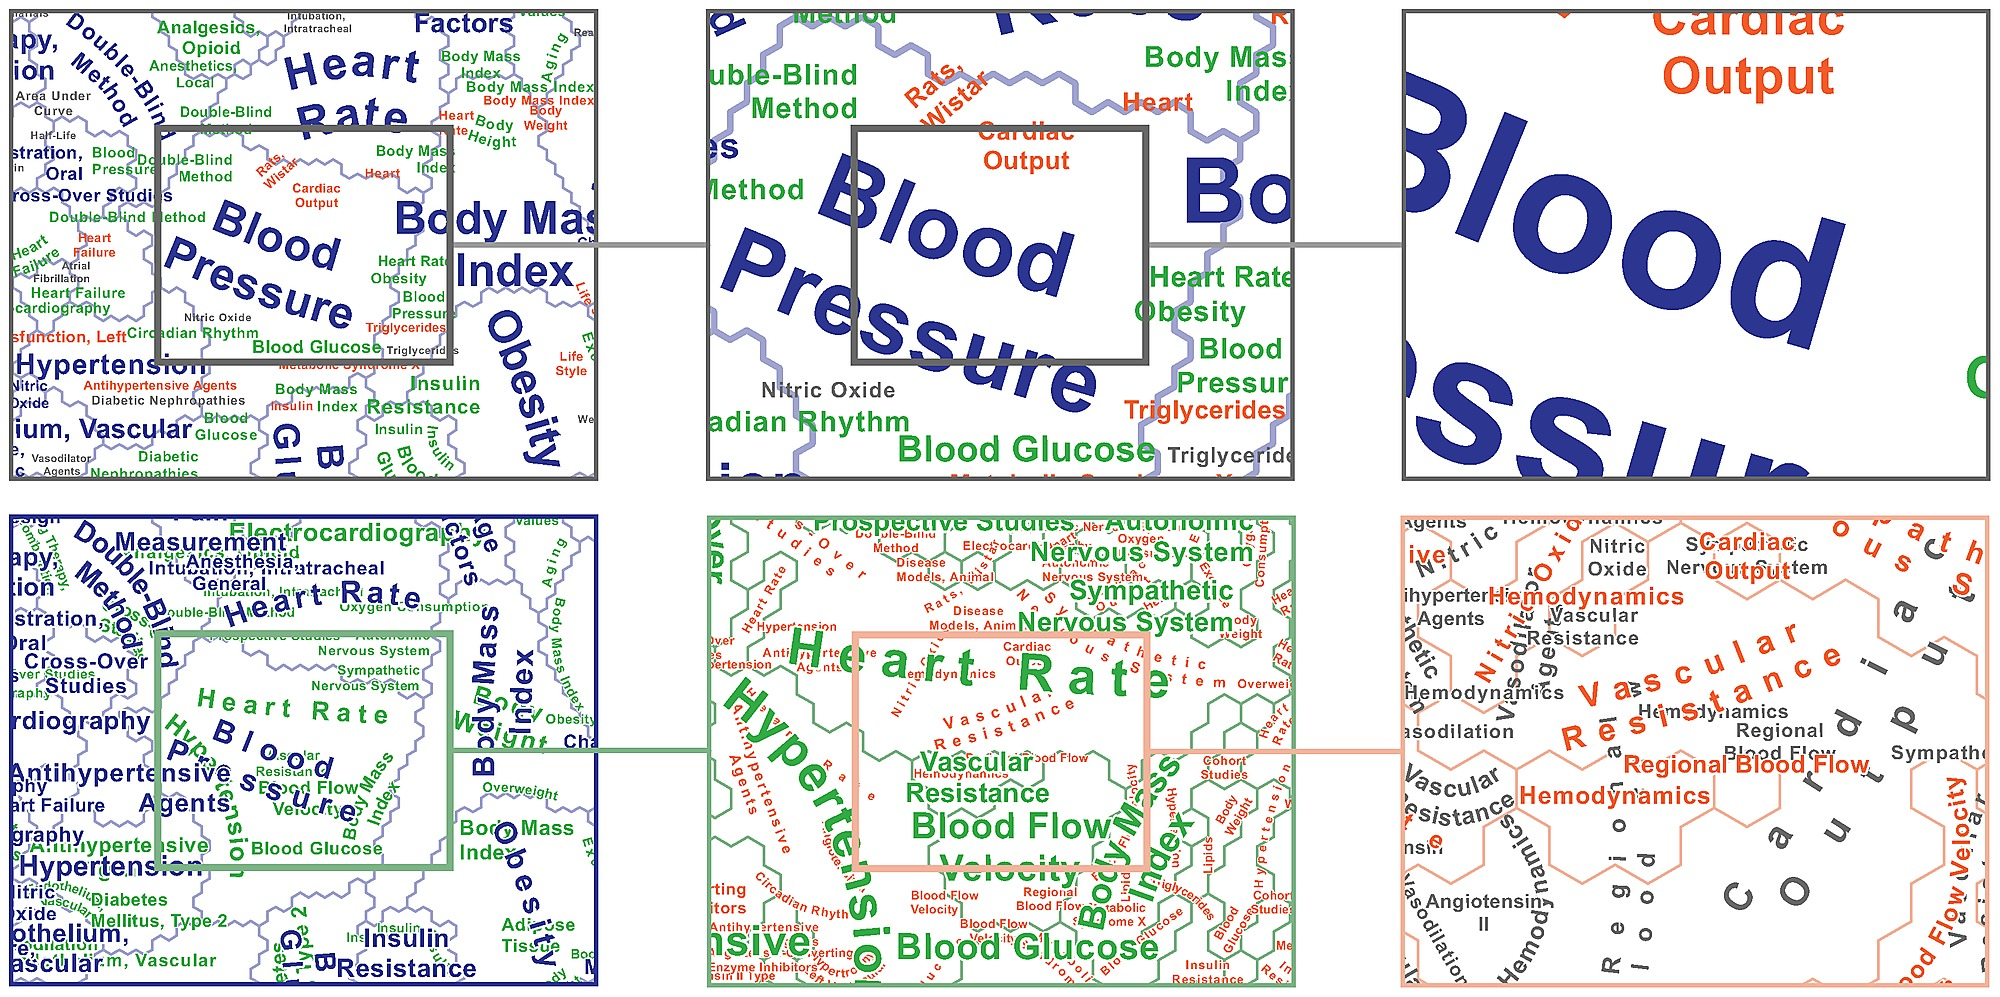
\includegraphics[width=\textwidth]{img/preview}
\caption{Geometric zooming (top) versus semantic zooming with successive revealing of lower levels of term dominance (bottom). Source: \cite{Skupin2013}}
\label{fig:som}
\end{sidewaysfigure}

One can observe that in semantic zooming, the level of detail increases with the zoom level.
Specifically, finer subareas with own labels and boundaries become visible.
Unfortunately, the zooming itself is not implemented in an interactive way in Skupin's case.
Instead, static images are pre-rendered for specific zoom levels.
Deciding when to switch between different levels of detail is a separate problem that we address in our work as described in \autoref{subsec:hierarchical_clustering}.

\subsubsection{Brushing and linking}
\label{subsubsec:brushing_and_linking}

``\textit{Brushing and linking} refers to the connecting of two or more views of the same data, such that a change to the representation in one view affects the representation in the other views as well''  - \cite{hearst1999modern}. 
Multiple views of the same data are usually implemented via different types of visualizations.
Common examples include combinations of scatter plots, bar charts, parallel coordinate views and maps.
Charts do not necessarily need to be of different types.
They may show different dimensions of the data instead (see \autoref{fig:correlation_matrix}).

\begin{figure}[!]
\centering
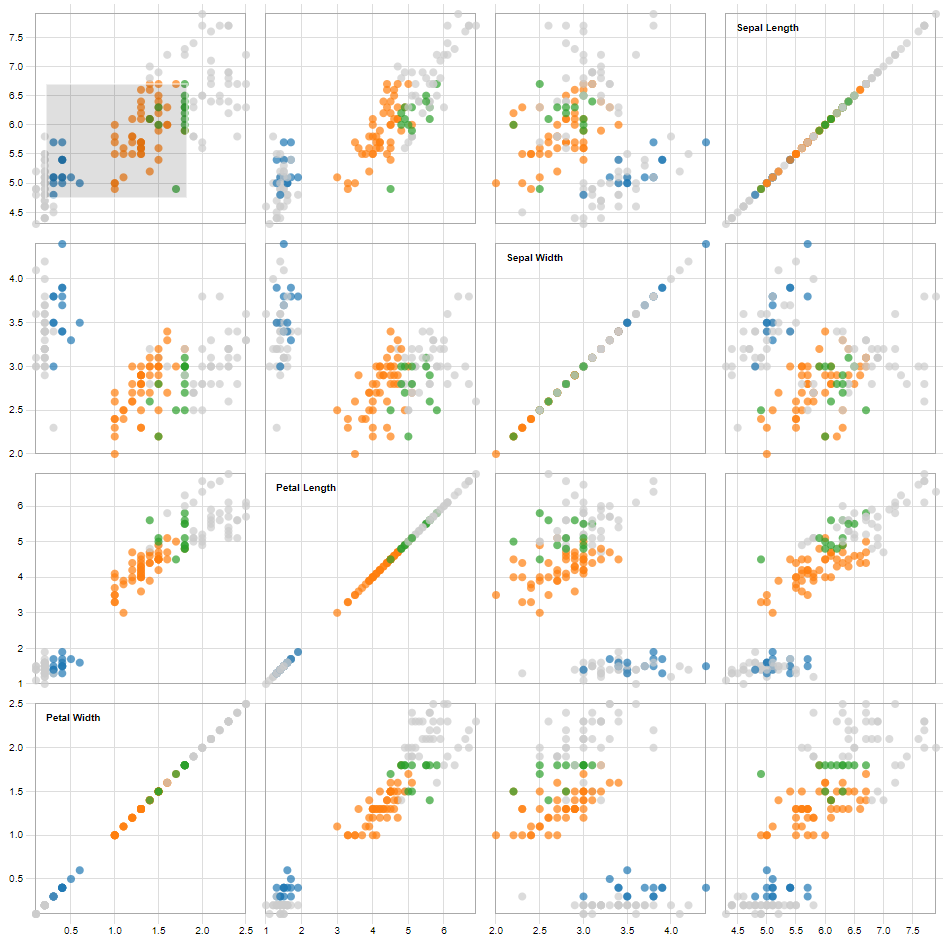
\includegraphics[width=\textwidth]{img/correlation_matrix}
\caption{Correlation matrix of a well-known Iris dataset as an example of brushing and linking. Linked views are all of the same type, which in this case is a scatter plot. Brushed view is in the upper-left corner. Image source and demo: \cite{Bostock2019a}}
\label{fig:correlation_matrix}
\end{figure}

\textit{Brushing} means selecting a part of the data in one of multiple views. 
A selection area is usually formed by dragging the cursor, hence the name \textit{brushing}.
Some form of visual indication is necessary to prevent confusion about what exactly has been selected.
\textit{Linking} refers to highlighting the selected data points in other view or views.
The data is ``linked'' through the selection.
A schematic example of coordinated views with brushing and linking can be seen in \autoref{fig:brushing_linking}.

\begin{figure}[!]
\centering
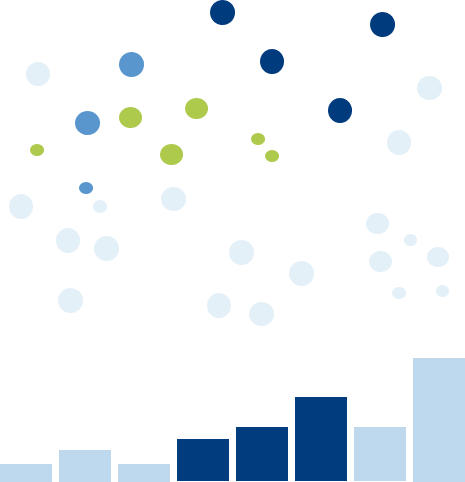
\includegraphics[width=0.4\textwidth]{img/brushing_linking}
\caption{A histogram and a scatter plot coordinated through brushing and linking. The data points that do not belong to the current selection are grayed out in both views.}
\label{fig:brushing_linking}
\end{figure}

\subsection{Machine learning}
\label{subsec:machine_learning}

\subsubsection{Word2vec}
\label{subsubsec:word2vec}

Word2vec was proposed by Mikolov \cite{Mikolov2013}. 
It is a neural network architecture for computing continuous vector representations of words in an n-dimensional space.
The model learns to predict words based on their context.
With enough training data, the hidden layer learns that semantically similar words can be represented with similar vectors.
Those word representations are called \textit{word embeddings} and typically have between 100 and 300 dimensions, while less than 50 dimensions usually don't represent the semantics well enough.

Semantic relationships expressed by word embeddings can be of multiple types.
\cite{Mikolov2013} evaluated semantic and syntactic relationships in question-answer pairs such as city-in-state (i. e. Chicago - Illinois), man-woman (i.e. brother - sister), opposite (ethical - unethical), nationality-adjective (Switzerland - Swiss).
If two words are close in the embedding space, it might also mean that they are synonyms or often appear together in texts.
An illustrative overview of concepts behind word2vec, its training and parameters can be found in \cite{Alammar2019}.

\subsubsection{\gls{tsne}}
\label{subsubsec:tsne}

\gls{tsne} is a dimension reduction technique proposed by \cite{LaurensvanderMaaten2008}.
The aim of the technique is to map high-dimensional data to a two- or three-dimensional space.
At the same time, the structure of the high-dimensional data should be preserved as much as possible.
In other words, \gls{tsne} defines a probability distribution in high-dimensional space and tries to preserve it for low-dimensional space using \textit{gradient descent}.
Gradient descent is an iterative optimization algorithm which aims to find a minimum of a function by taking small steps in the direction of the steepest decline.
The optimization is initialized randomly and is in the case of \gls{tsne} defined by a non-convex cost function, which means that risk of getting stuck in local minima exists.
It is, however, completely acceptable to run the algorithm multiple times and choose the best result.
\gls{tsne} succeeds in preserving both global and local structure of the data, which makes clusters visible at several scales.
An excellent interactive overview of \gls{tsne}'s parameters (especially perplexity) and their influence on resulting behavior of the algorithm can be found in \cite{wattenberg2016how}.

\subsection{Definitions from the patent domain}
\label{subsec:definitions_from_the_patent_domain}

This section contains some basic knowledge about the patent system which is a prerequisite for an understanding of the patent visualization tools related to this work (described in \autoref{sec:state_of_the_art}), and also for an understanding of our own approach (described in \autoref{ch:concept}).
We show how patent documents are structured. 
We also define some terminology from the patent domain that we use throughout this work: patent family, citations and \gls{ipc} classes.

\subsubsection{Structure of a patent document}
\label{subsubsec:structure_of_a_patent_document}

Each patent document possesses the following attributes:
\begin{itemize}
\item \textit{Application number} -  a unique identifier, starts with country code of the registration country. Example: US-5448677-A.
\item \textit{Country code} - stands for the code of the patent office the application was submitted to. 
While some countries, like the US, have their own designated patent offices, there are patent offices, such as the European Patent Office, that allow patents to be valid in multiple countries.
In those cases, terrestrial validity of patents is a complex topic.
For the purposes of simplification, we only consider the code itself (e.g. US or EP) in this work.
\item \textit{Priority date} - the date when the priority patent was submitted (see \autoref{subsubsec:patent_family_and_priority_document} for details on priority).
For our purposes this date is considered as the creation date of the patent.
\item \textit{Assignees} - a list of one or many individuals (inventors) or institutions to which the rights to the invention belong to. It is a categorical attribute.
\item \textit{\gls{ipc} classes} - a list of one or many codes from the \gls{ipc} classification (see \autoref{subsubsec:ipc_classification} for more details) describing the thematic areas of technology the described invention is related to. It is a categorical attribute of a hierarchical nature.
\item \textit{Citations} - a list of patents (identifiable by their application numbers) cited by the given document.
\item \textit{Family identificator} - a number that all members of one patent family share.
\item \textit{Title} - a text attribute describing the invention very briefly . It often does not contain enough useful information if used by itself, but adds some clarity when combined with the abstract.
\item \textit{Abstract} - by analogy with scientific publications, it is a brief summary of the invention.
\item \textit{Claims} - detailed description of the invention and its aspects that should be protected (claimed) by a patent.
This is the field with the most textual information as it can be hundreds to thousands of words long.
Our main data source, Google Patents Public Datasets \cite{IanWetherbee2017}, only provides claims for patents registered in the US.
\end{itemize}

This list is not extensive and only includes fields that are relevant to this work.
For the above-described fields, we distinguish between \textit{textual content} of a document (title, abstract and claims) and the \textit{metadata} which includes all remaining information.

\subsubsection{Patent family and priority document}
\label{subsubsec:patent_family_and_priority_document}

Patents can be assigned to the same \textit{patent family}.
Protection of intellectual property for a patent is restricted to the country the application was submitted to.
Therefore, many inventions are registered in patent offices in multiple countries.
The patents covering one invention across several countries constitute a family.
The earliest patent from a family is called a \textit{priority document}.
Families can also be registered in the same country when they describe different aspects of the same invention.

\subsubsection{Forward and backward citations}
\label{subsubsec:forward_backward_citations}

A patent may include a list of tens to hundreds of citations defined by their application numbers.
When a new patent application cites an already existing patent, it indicates that the cited patent is already known to the applicant \cite{Cotropia2013}.
The older patent in this case is considered \textit{prior art}. 
The new application must provide claims that are novel and non-obvious in the view of the prior art. 
It is in the interest of the applicant to show (through a citation) that they have thoroughly studied already existing patents.
This is analogous to scientific publications where the authors have to review state-of-the-art before proposing novel approaches.

The citations directly defined in a patent, i. e. links to older documents that are being \textit{cited}, are called \textit{forward citations}.
\textit{Backward citations} are the same links from the point of view of the older patent.
They show the patents \textit{citing} the current one.
As it is impossible to know how a patent will be cited in the future, an explicit list of backward citations does not exist and has to be assembled by reversing forward citations.

\subsubsection{International Patent Classification}
\label{subsubsec:ipc_classification}

Each patent is assigned at least one, but usually multiple \gls{ipc} codes.
The \gls{ipc} hierarchy breaks the whole of humanity's patented technological knowledge down into thematic areas the inventions pertain to.
One \gls{ipc} class is an alphanumerical code which is hierarchical in nature and is based on prefixes, i. e. it starts with one letter and with addition of further symbols corresponding new nodes in the hierarchy tree appear.
The tree structure is of the constant depth of five levels and, as we learned in the expert interviews (described in \autoref{subsec:implications}), those levels have own names and are composed according to certain rules (see \autoref{table:ipc_classes_structure}).

\begin{table}[h!]
\centering
\begin{tabular}{||l l l l||} 
 \hline
 Name & Format & Example & Example title \\ [0.5ex] 
 \hline\hline
 Section & One letter & H & Electricity \\ 
 Class & Two-digit number & H04 & Electric communication technique  \\
 Subclass & One letter & H04N & Pictorial communication, e.g. television \\
 Group & One-to-three-digit number & H04N5 & Details of television systems \\
 Subgroup & Two- or three-digit number & H04N5/76 & Television signal recording \\ [1ex] 
 \hline
\end{tabular}
\caption{Structure of \gls{ipc} classes}
\label{table:ipc_classes_structure}
\end{table}

\section{State-of-the-art visualization approaches}
\label{sec:state_of_the_art}

After all prerequisite concepts have been introduces, we review the state of the art with regard to explorative visualization approaches.

Federico et al. \cite{Federico2017} surveyed 21 existing visualization approaches for patents and 109 for scientific documents such as papers, focusing on non-commercially available tools. 
They distinguish between four data types that can be visualized: \textit{text}, \textit{citations}, \textit{authors} and \textit{metadata}.
We focus our review of state-of-the-art on approaches that visualize 1) text alone, 2) other data types alone and 3) text in combination with other data types.
A separate section is devoted to a group of comparable themescape-based approaches.
In the following, a selection of works discussed by Federico et al. is expanded by some other approaches which they did not include.

\subsection{Text-based visualizations}

Johnson et al. \cite{Johnson} present a similar visualization approach to ours with regard to processing the text data for the visualization. 
They use a word2vec model trained on ca. 1.5 million patent texts and compose document embeddings through averaging of word embeddings as well.
They, however, only focus on textual content and disregard visual representation of metadata.
An overview of the whole dataset is not provided.
Instead, one needs to query the data by keywords and only subset corresponding to the query is then shown (see \autoref{fig:johnson}.
The only interaction available apart from querying is the selection of a single patent by clicking on the corresponding point, so that patent details are displayed.
The approach proposes no method to automatically label data points to provide an overview.

\begin{figure}[!]
\centering
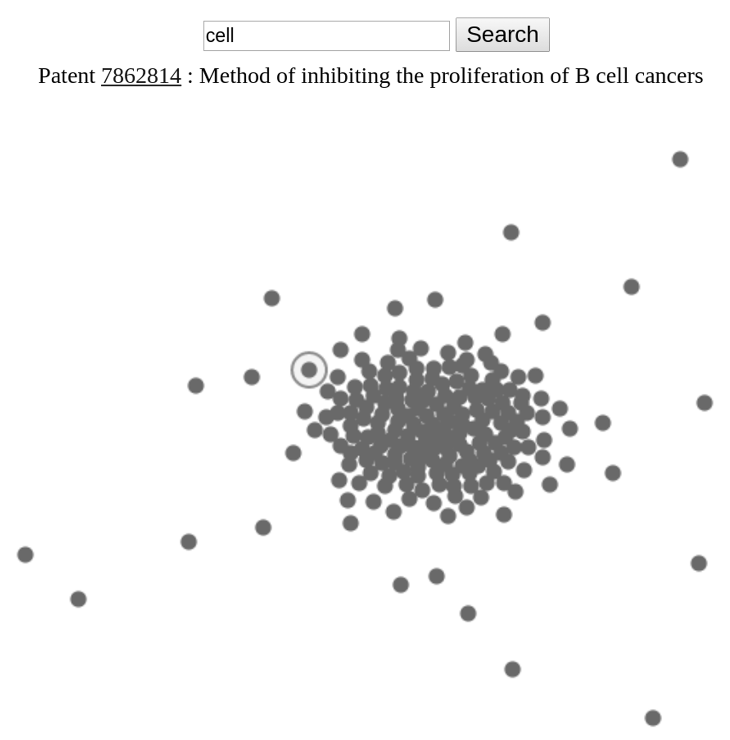
\includegraphics[width=0.5\textwidth]{img/johnson}
\caption{The visualization proposed by \cite{Johnson}. Output of a query for ``cell''. The point in a circle shows the currently selected patent.}
\label{fig:johnson}
\end{figure}

Skupin \cite{Skupin2002} \cite{Skupin2004a} applies a cartographic approach to create maps of non-geographic information, more specifically, conference abstracts.
In a successor work (see Figure \autoref{fig:skupin}), Skupin et al. \cite{Skupin2013} visualize medical publications based on MeSH terms, which are analogous to tags assigned to scientific articles.
In all of those works, a type of \gls{ann} called \gls{som} is used. 
The network is trained on a term-document-/MeSH-document matrix. 
This way, each neuron is assigned multiple terms as labels.
In \cite{Skupin2013}, the neurons are then clustered in the following way: ``if two neurons are neighbors in the two-dimensional neuron lattice and they share the same top-ranked label term, then their boundary is dissolved, thus forming a larger polygon, a neuron label cluster'' \cite{Skupin2013}.
The same procedure is duplicated for the second and third top-ranked label terms, and the resulting three clusterings are then overlaid on the same map and distinguished by color.
Cluster size declines with the dominance of the term, which means the end result displays multiple levels of semantic detail.

\begin{figure}[!]
    \centering
    \subfigure[Zoomed-out view of a complete map of medical literature and detailed views of some regions. Blue, green and red labels indicate clusters derived from the first, second and third top-ranked label term, respectively. Source: \cite{Skupin2013}]
    {
        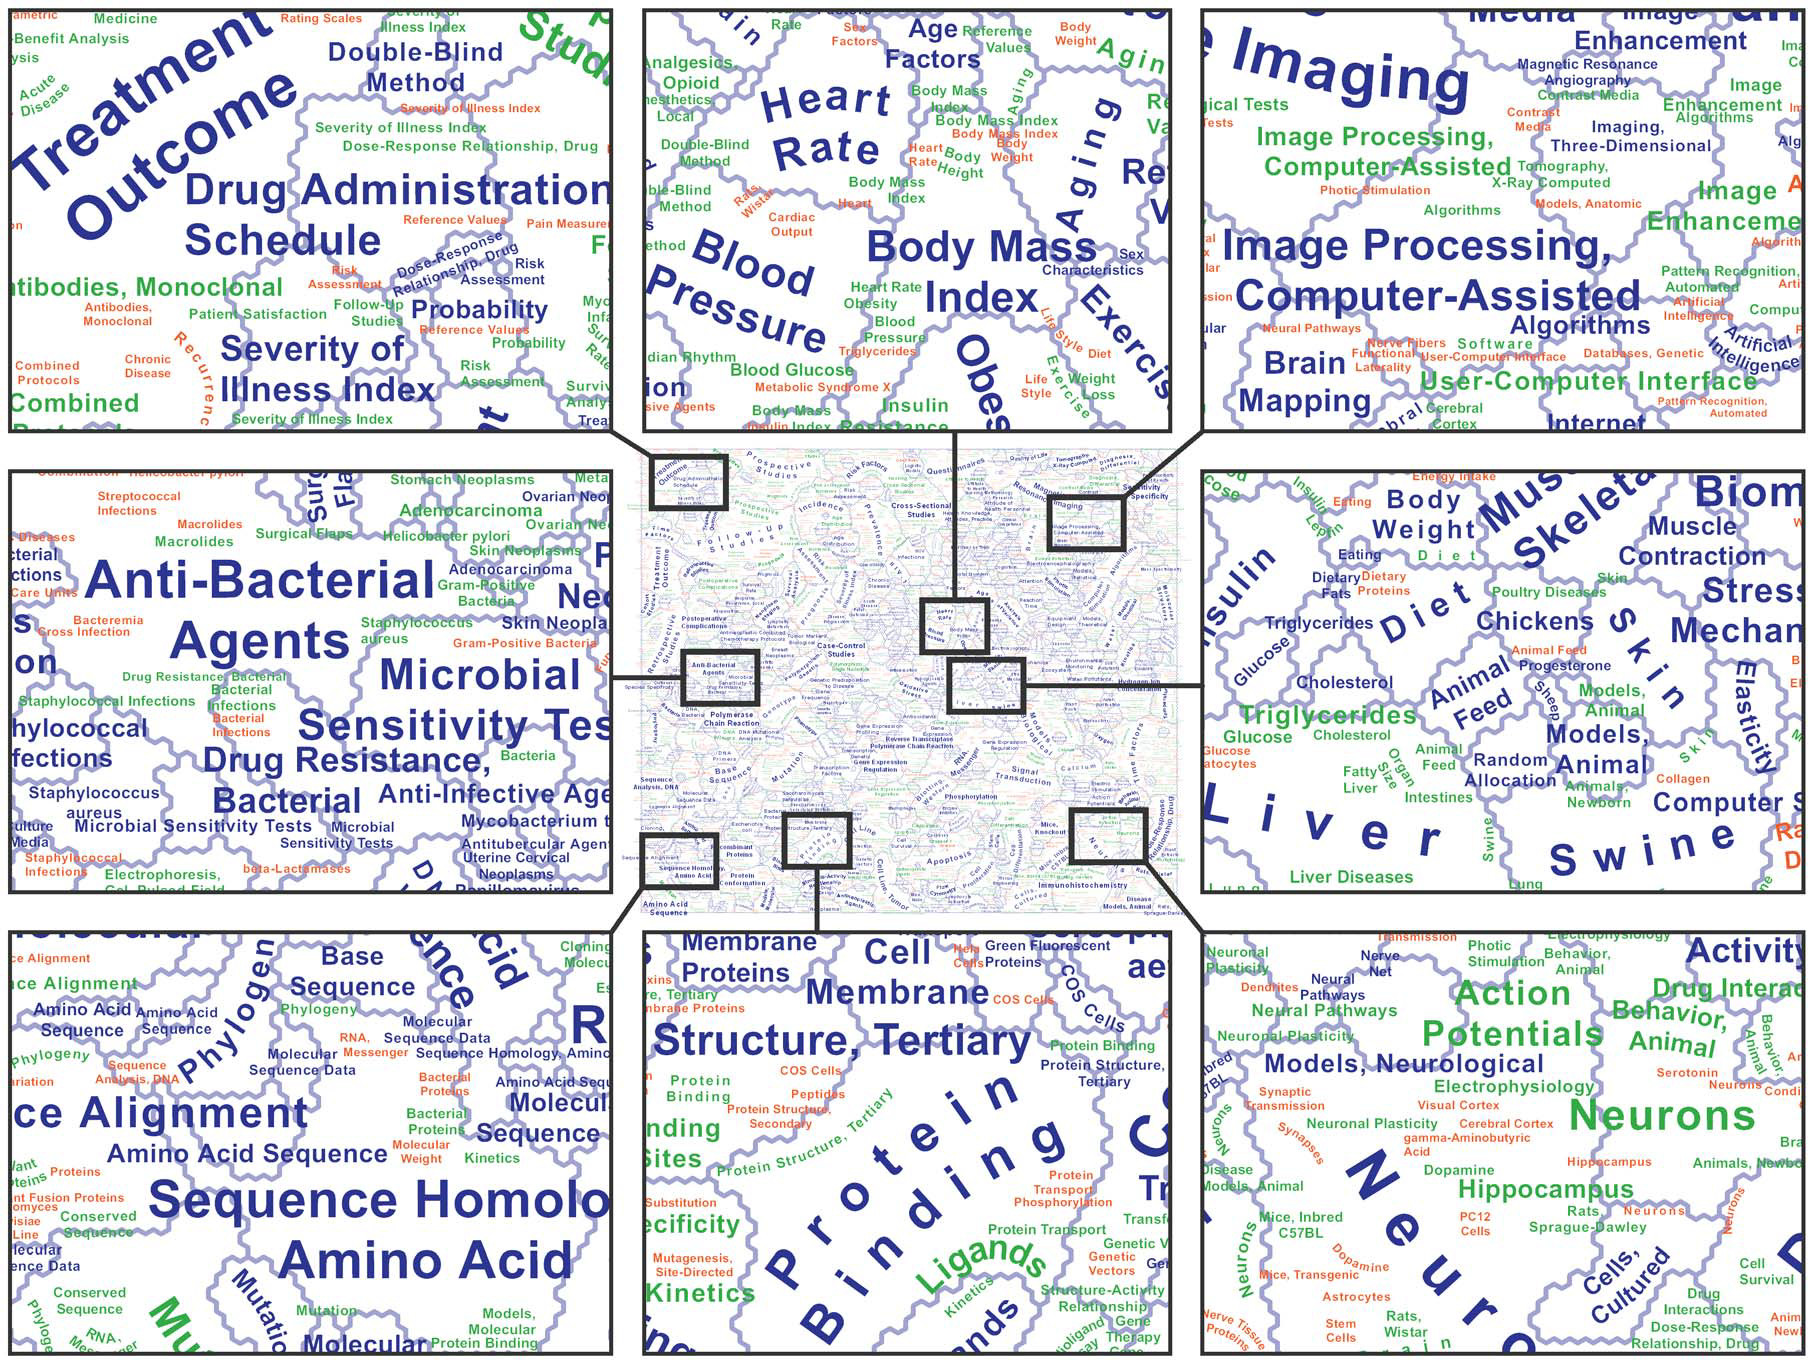
\includegraphics[width=\textwidth]{img/skupin}
        \label{fig:skupin}
    }\\
    \subfigure[Visualization of conference abstracts with simultaneous overlay of three levels of a hierarchical clustering. Source: \cite{Skupin2002}]
    {
        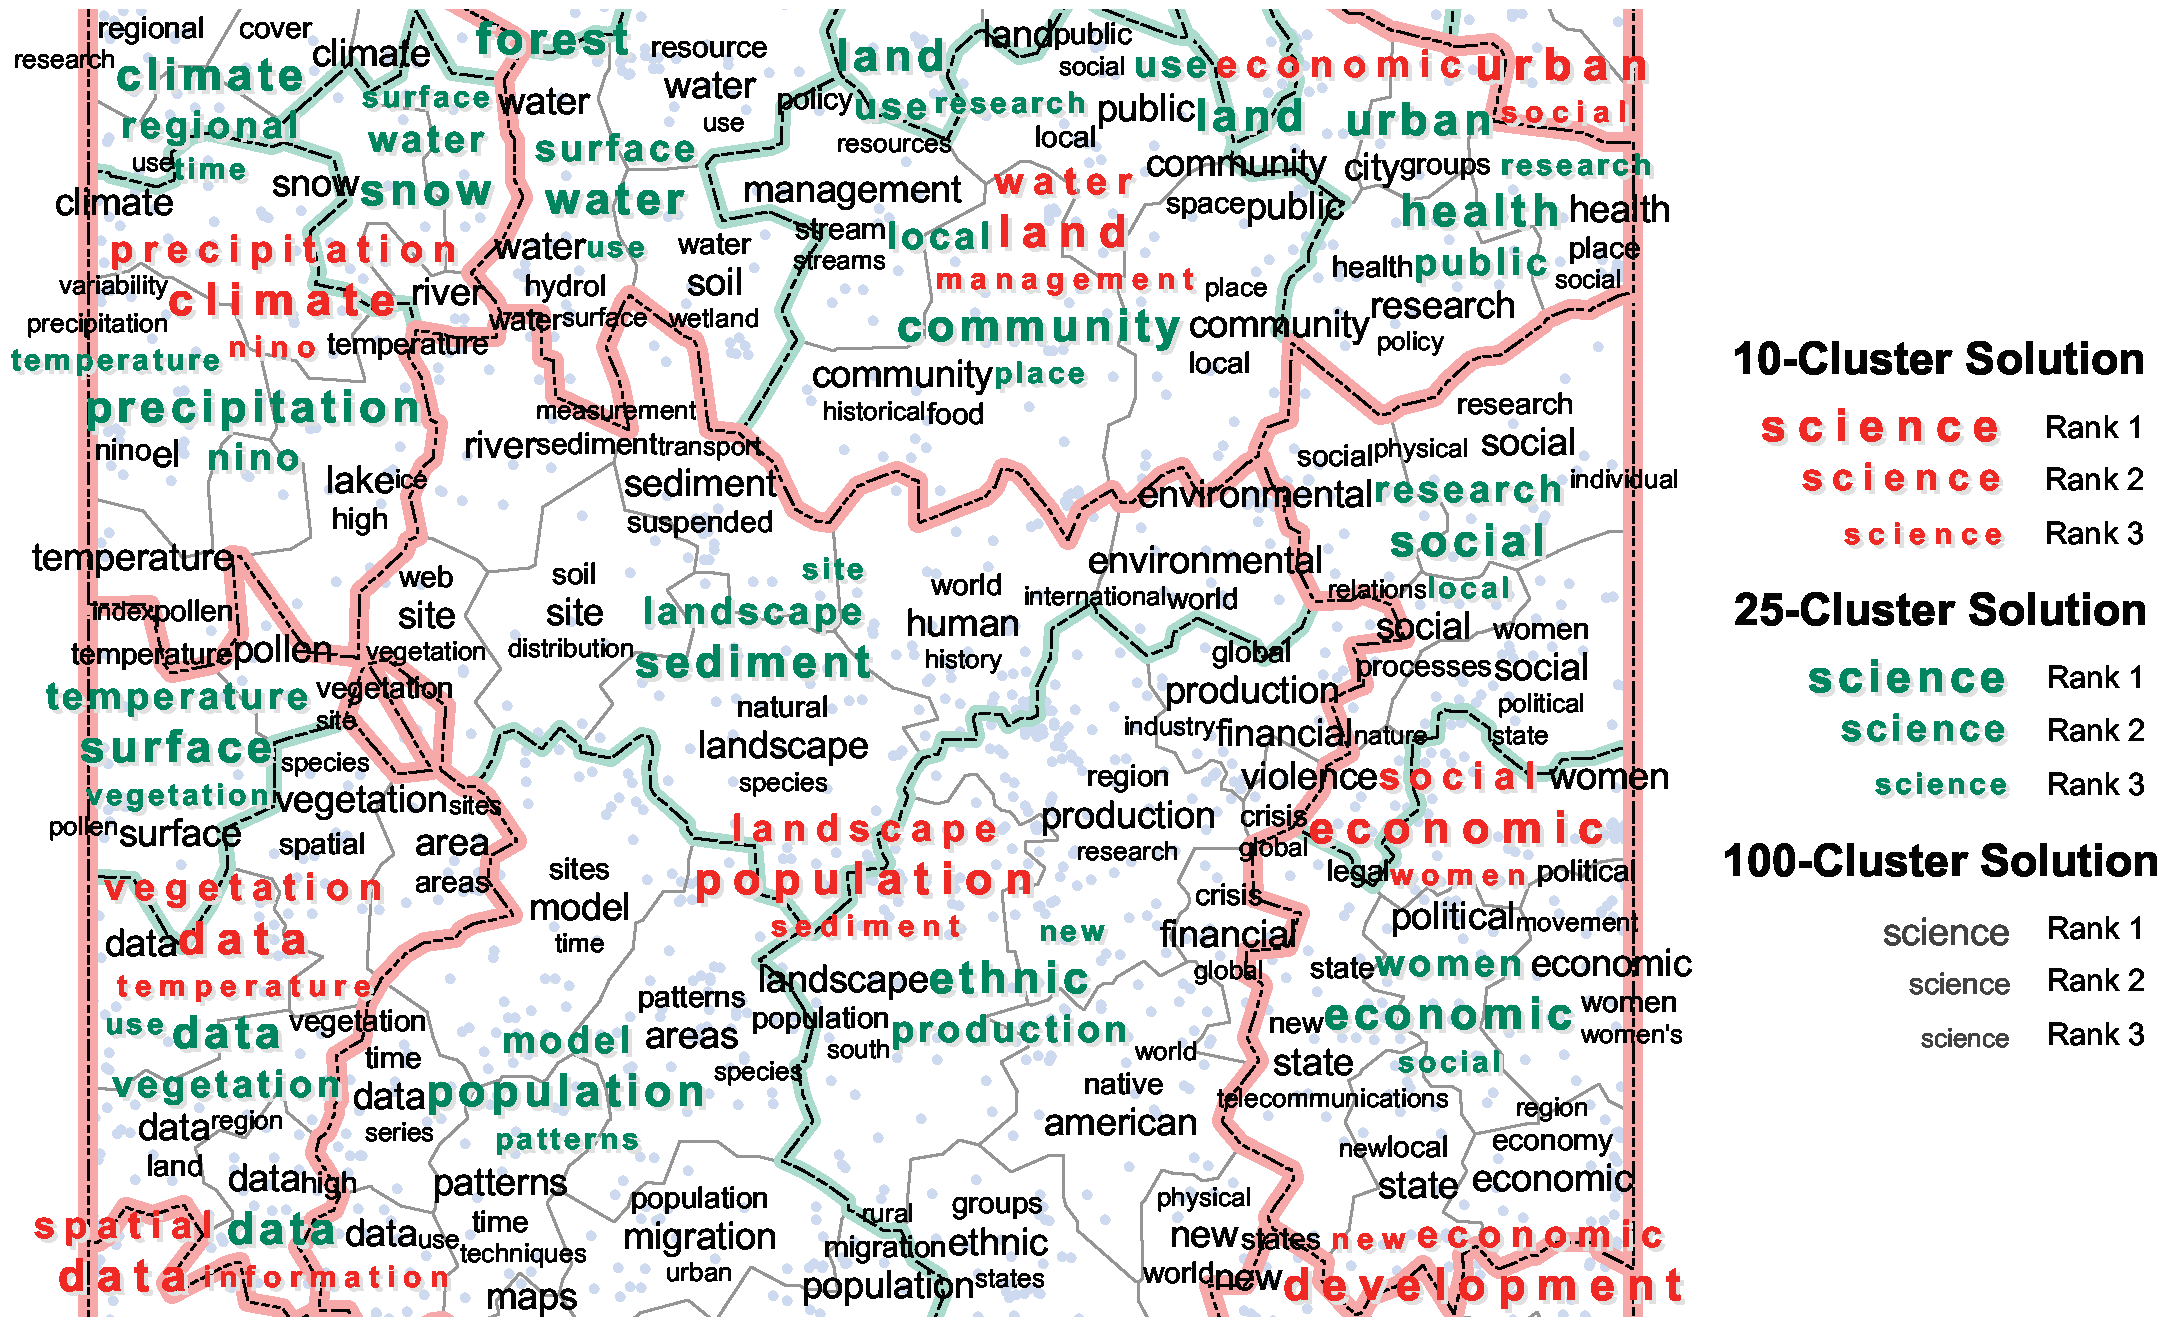
\includegraphics[width=\textwidth]{img/skupin1}
        \label{fig:skupin1}
    }
    \caption{Skupin's maps of knowledge domains}
    \label{fig:skupin_all}
\end{figure}

In \cite{Skupin2002} and \cite{Skupin2004a}, Skupin uses an alternative clustering method - hierarchical clustering.
From the tree structure built on neuron similarities he derives three to five clustering levels as shown in Figure \autoref{fig:skupin1}.
This approach served as an inspiration for our own hierarchical clustering based on similarities between patent documents.

Our approach builds upon Skupin's ideas and aims for a comparable result, while the features of the data and the processing methods are different.
Visualizations proposed by him are either static or provide a basic zooming interaction while limiting the richness of display.
We, on the contrary, specifically focus on supplementing a hierarchical themescape with interactivity for effective exploration.

Choo et al. \cite{utopian} present UTOPIAN (\textbf{U}ser-driven \textbf{T}opic modeling based on \textbf{I}nter\textbf{a}ctive \textbf{N}onnegative Matrix Factorization).
They perform topic modeling based on a bag-of-words representation of a document.
A hard-clustering algorithm is then applied to the documents, which means that each document is assigned to only one topic.
A modified version of \gls{tsne} is utilized to draw a node-link diagram with topics/clusters distinctly separated as shown in \autoref{fig:utopian}.
Edges are drawn between pairs of data points whose distances are below a user-specified threshold.
Most importantly, the approach gives the user a high level of control over the topic modeling result.
Merging or splitting topics, creation of a new topic based on a specified document or a certain keyword are possible.
Choo's approach influenced our initial idea of drawing a fully connected graph of documents which would dynamically reform itself after some documents are filtered out (see \autoref{subsec:initial_concept} for details).
We, however, did not pursue this idea further because of performance considerations.

\begin{figure}[!]
\centering
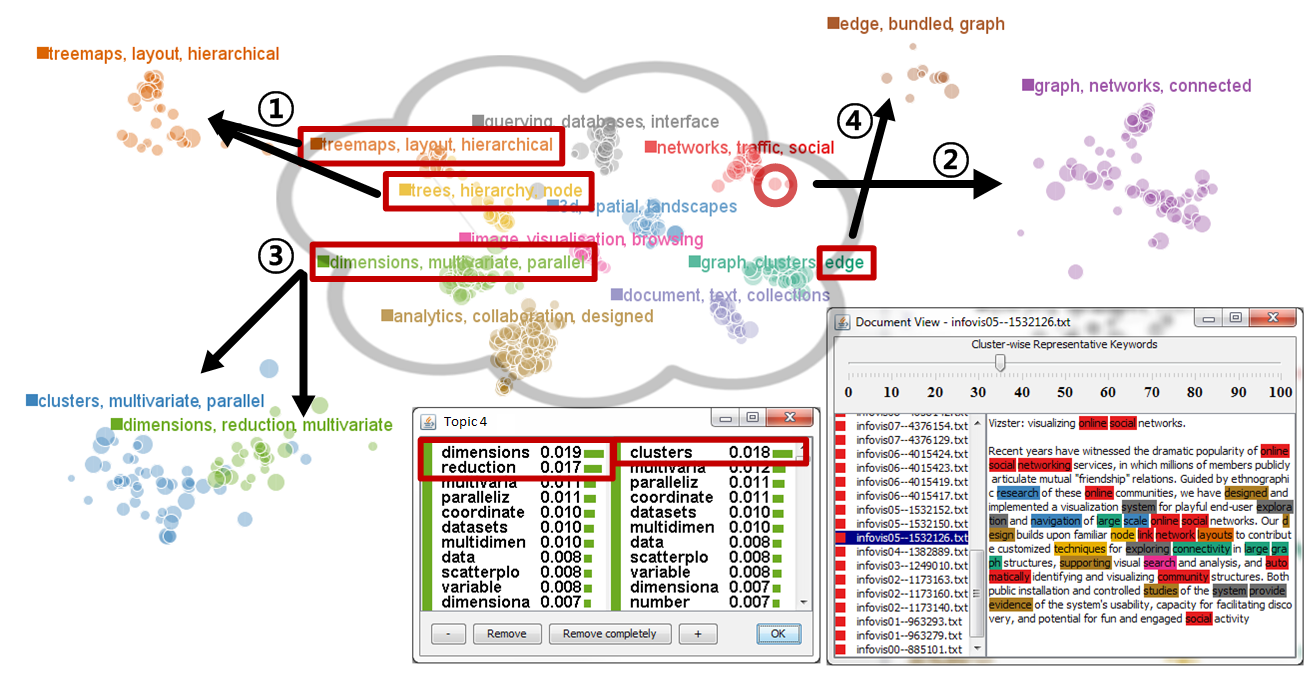
\includegraphics[width=\textwidth]{img/utopian}
\caption{UTOPIAN by \cite{utopian}. Given a scatter plot visualization generated by a modified \gls{tsne}, it provides capabilities for 1) topic merging, 2) document-induced topic creation, 3) topic splitting and 4) keyword-induced topic creation. The user can adjust topic keyword weights (bottom-middle) and see representative keywords in the document viewer (bottom-right).}
\label{fig:utopian}
\end{figure}

\subsection{Visualizations based purely on metadata}

Patent data is distinguished by a significant amount of metadata attached to each record: hierarchical classification, assignees, citations, patent family information, etc.
Many works deal with one or a number of these attributes \cite{Zhao2013} \cite{Wittenburg2015} \cite{Herr2014a} \cite{Giereth2007} \cite{Garfield2004} \cite{Chen2004} \cite{abello}.
However, Federico et al. emphasize that “only few works adopt, refine, or develop techniques for visualizing classification data. Other data types are just ignored in most approaches” \cite{Federico2017}.
Because of this, we aim to derive value specifically from the hierarchical representation of \gls{ipc} classification data.

Wittenburg et al. \cite{Wittenburg2015} make extensive use of metadata for faceted visualization with what they call embedded bar charts.
They order the company, decade of filing date, country and \gls{ipc} class vertically over each other and represent the distribution of values within those attributes through widths of blocks as seen on \autoref{fig:wittenburg}.
The embedded bar charts use negative space within the blocks to display temporal development of a company's patenting behavior.
Unfortunately, Wittenburg's approach results in a cluttered view and therefore lacks visual scalability when many companies and especially \gls{ipc} classes are present in the data.
Nevertheless, we build upon their idea about displaying distributions of metadata attributes in a stacked order.

\begin{figure}[!]
\centering
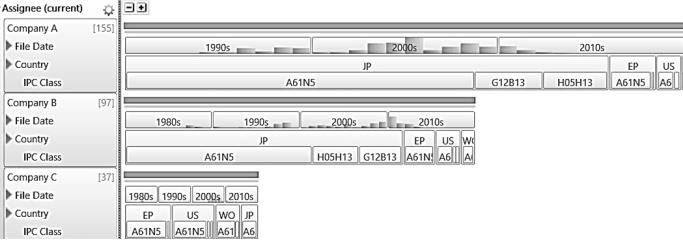
\includegraphics[width=\textwidth]{img/wittenburg}
\caption{A visualization layout proposed by \cite{Wittenburg2015}, a so called embedded bar chart. The distribution of metadata attributes in the dataset is represented by a hierarchy of attributes: assignee, then date of filing, then country, then \gls{ipc} class.}
\label{fig:wittenburg}
\end{figure}

\subsection{Visualizations based on text in combination with other data types}

%User interaction provides immense added value in the task of finding patterns in data. 
%However, Federico et al. note that most visualizations only made limited use of interaction techniques such as detail-on-demand, focus + context or coordinated multiple views. 
%This research gap needs to be addressed specifically because interaction plays a big role in tackling the challenge of scalability for the steadily increasing number of text documents.

Many approaches capture thematic similarities between documents with help of topic modeling \cite{nakazawa} \cite{gretarsson} \cite{Dou2011} \cite{Jiang2016}.
They position a document depending on the degree to which it belongs to the corresponding topic.
For example, Dou et al. \cite{Dou2011} uses the parallel coordinate metaphor to present a probabilistic distribution of a document across pre-detected topics as seen in \autoref{fig:dou}.
With an interactive ThemeRiver view they present the temporal development of the topics.
Lastly, they use a scatter plot to show the distribution of single-topic vs. multi-topic documents.
Pie glyphs within the scatter plot describe the topical contribution to a specific document.
We consider the parallel coordinate plot a suboptimal choice to represent a large number of similar dimensions such as >10 topics.
Even though the topic axes are ordered by similarity, the positive and negative correlations between topics become spread over the >10 vertical axes, which makes them hardly perceptible.
Nevertheless, this approach served as an inspiration for our own glyphs in the form of a pie chart.

\begin{figure}[!]
\centering
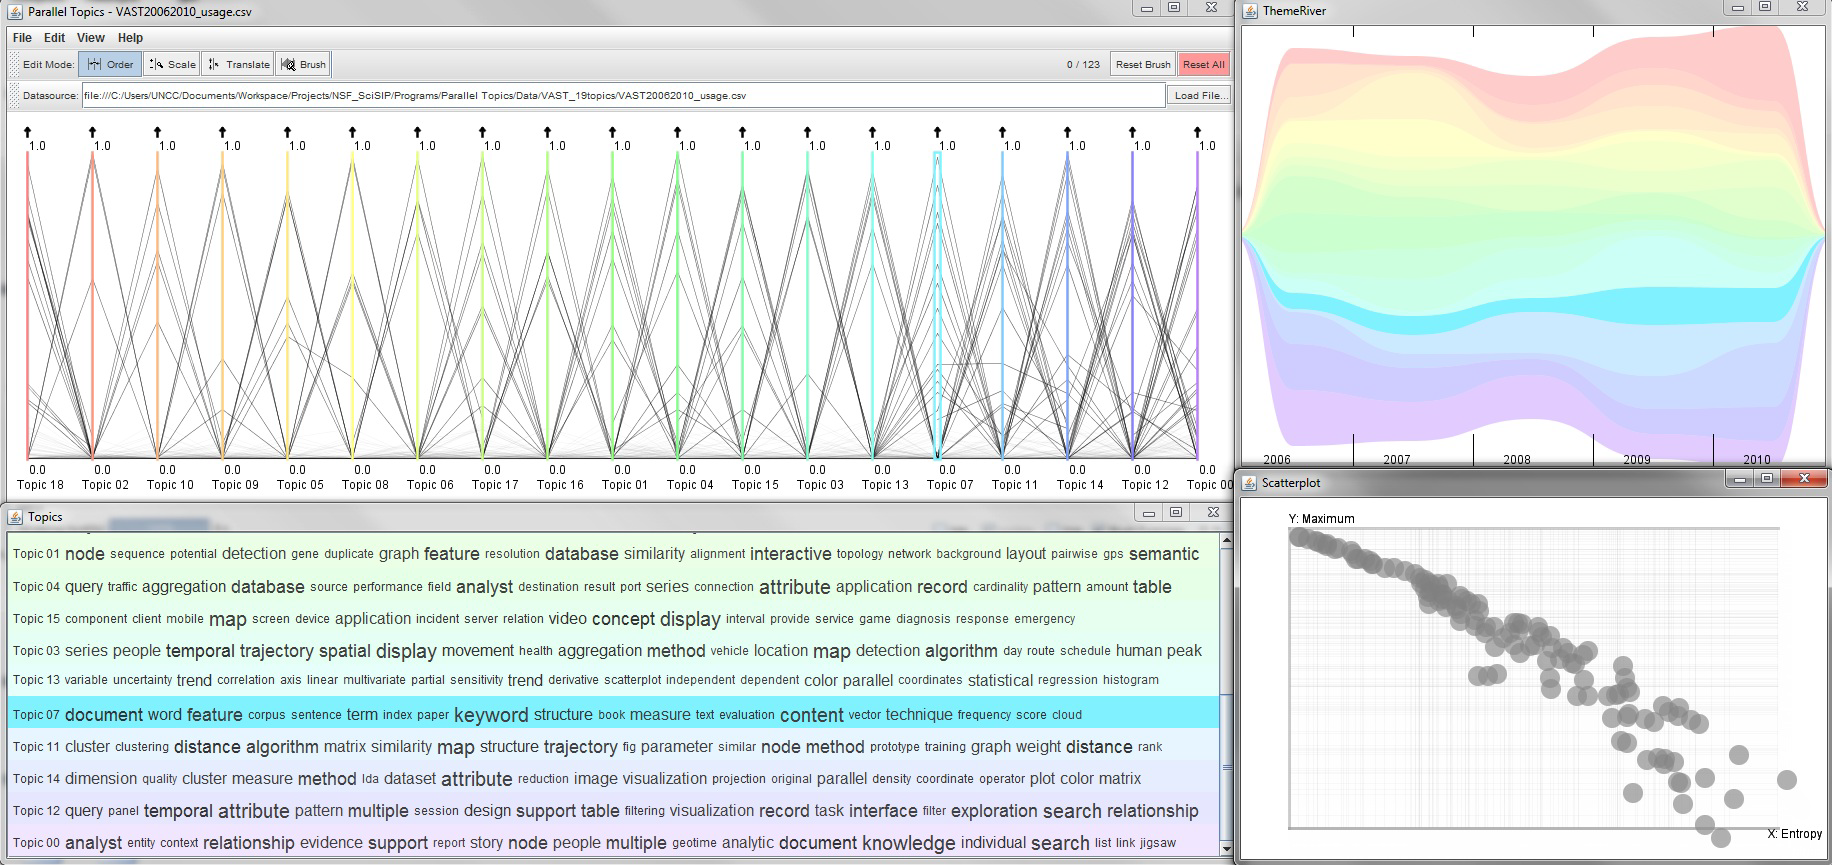
\includegraphics[width=\textwidth]{img/dou}
\caption{ParallelTopics by \cite{Dou2011}. Top left: Document Distribution view, top right: Temporal view, bottom left: Topic Cloud, bottom right: Document Scatterplot.}
\label{fig:dou}
\end{figure}

Jiang et al. \cite{Jiang2016} present a comparable approach to Dou et al. as seen in \cite{fig:jiang}.
They detect tens of topics using a hierarchical topic model.
Each topic is then represented as a vocabulary-length feature vector where each dimension corresponds to the word's probability in a latent semantic space.
The topic vectors are then reduced to two dimensions via \gls{mds} and are shown in the form of a scatter plot.
This approach comes close to our idea of making patterns in the semantic space visible.
Unfortunately, it does not provide a representation of how separate documents relate to topics.
It also involves only the temporal dimension of documents and no as an addition to their textual content, no other metadata is represented.

\begin{sidewaysfigure}[!]
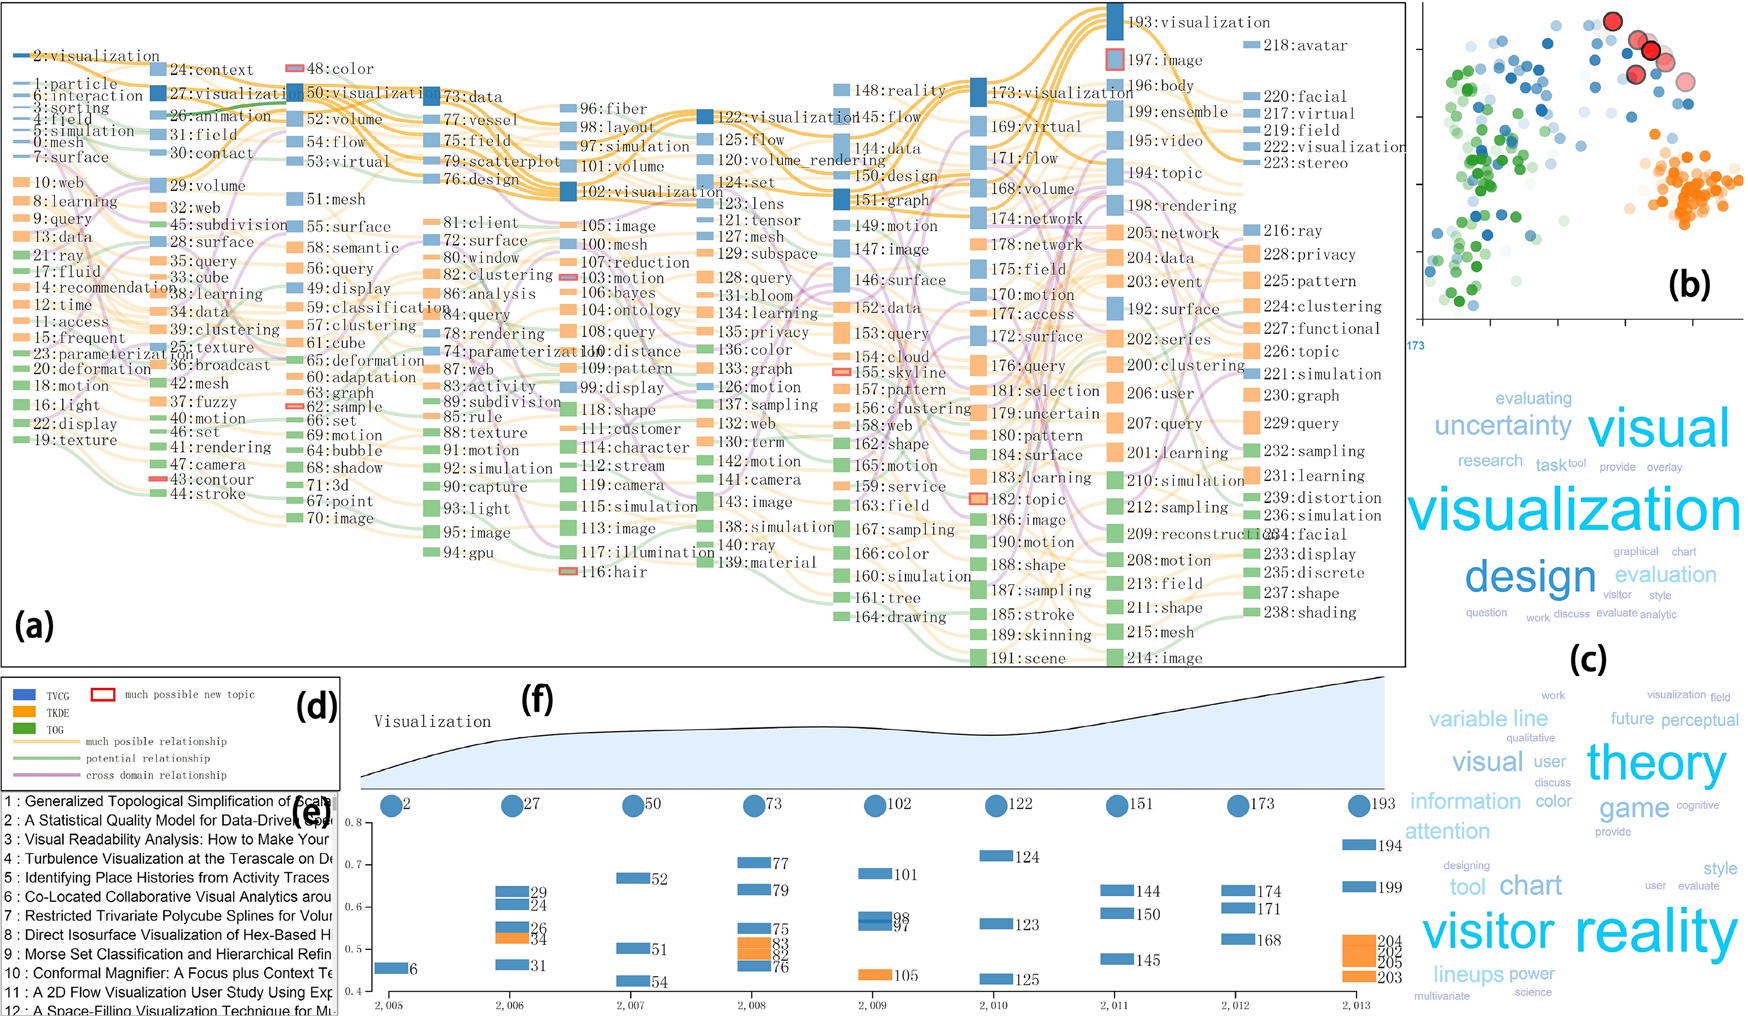
\includegraphics[width=\textwidth]{img/jiang}
\caption{A visualization approach by \cite{Jiang2016}. a) sankey diagram presenting the temporal development of numbered topics; b) scatter plot showing the topics in 2D space; c) word cloud of the selected topic and subtopics;  d) legend; e) titles of papers belonging to the selected topics; f) stream diagram illustrating the topic trend with a scatter plot to represent topic similarities. }
\label{fig:jiang}
\end{sidewaysfigure}

\subsection{Themescapes}
Visualization approaches that produce themescapes constitute a separate noteworthy category.
They include commercial tools such as VxInsight \cite{Boyack2002}, Thomson Reuter’s Aureka and STN's AnaVist.
Information about those tools is limited because of their cost, but \cite{Ruotsalainen2008} provides an extensive comparison.
There are also some non-commercial approaches such as IN-SPIRE \cite{hetzler}. 
All of those approaches utilize the metaphor of points in a landscape comprised of ``mountains'' and ``valleys'' as seen in \autoref{fig:aureka}.
Mountains group patents with similar textual content via word-frequency-based similarity metrics.
The height of a mountain peak corresponds to the document density in the area.
A peak is usually labeled with a list of automatically extracted relevant terms.
Skupin's work takes advantage of the map metaphor as well, but does not completely fit into this category because he does not use the third dimension to represent the amount of documents in a cluster.

In most themescape-based approaches, the user can highlight points on the landscape which correspond to a certain author, patent assignee, time period, country, etc.
Thus, a distribution of metadata values can be explored.
Moreover, coordinated views supplement the main landscape view by providing statistics in form of histograms, co-occurrence matrices, pie charts, citation graphs, etc. (see \autoref{fig:anavist} for an example from AnaVist).

The little information that is publicly available about the commercial themescape-based tools seems to indicate that all of them use document representations based on frequency and/or distribution of words.
In such classical machine learning methods, words are treated like indices in a dictionary and there is no concept of context or similarity between words.
In our work we compare one such approach (\gls{tf-idf} document vectors) with a newer neural-net-based approach that takes semantics of words into account.

\begin{figure}[!]
\centering
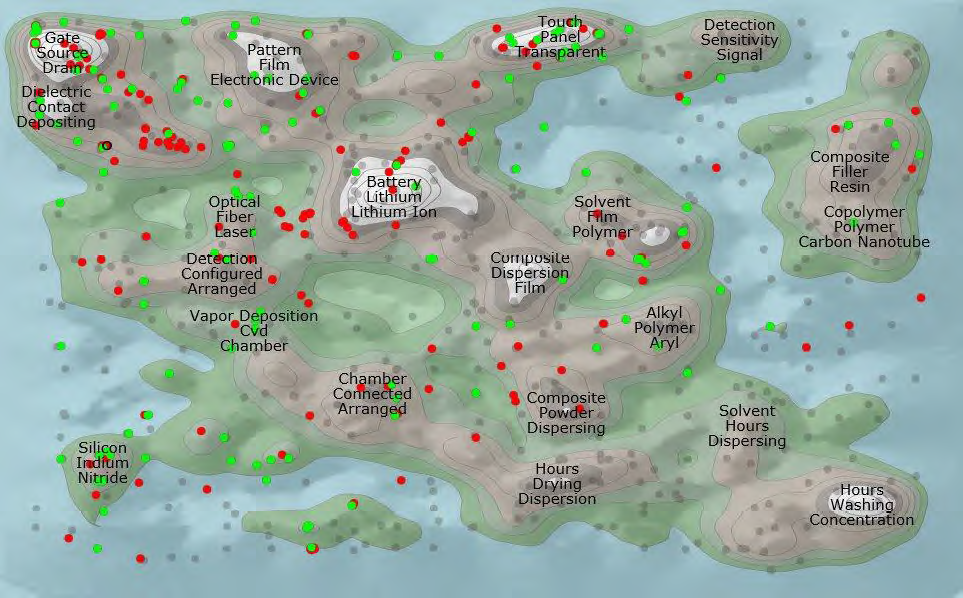
\includegraphics[width=\textwidth]{img/aureka}
\caption{A patent landscape map about graphene produced with Aureka. Highlighted are Samsung's patents published in 2013 and 2014. Image source: \cite{graphene}}
\label{fig:aureka}
\end{figure}

\begin{sidewaysfigure}[h!]
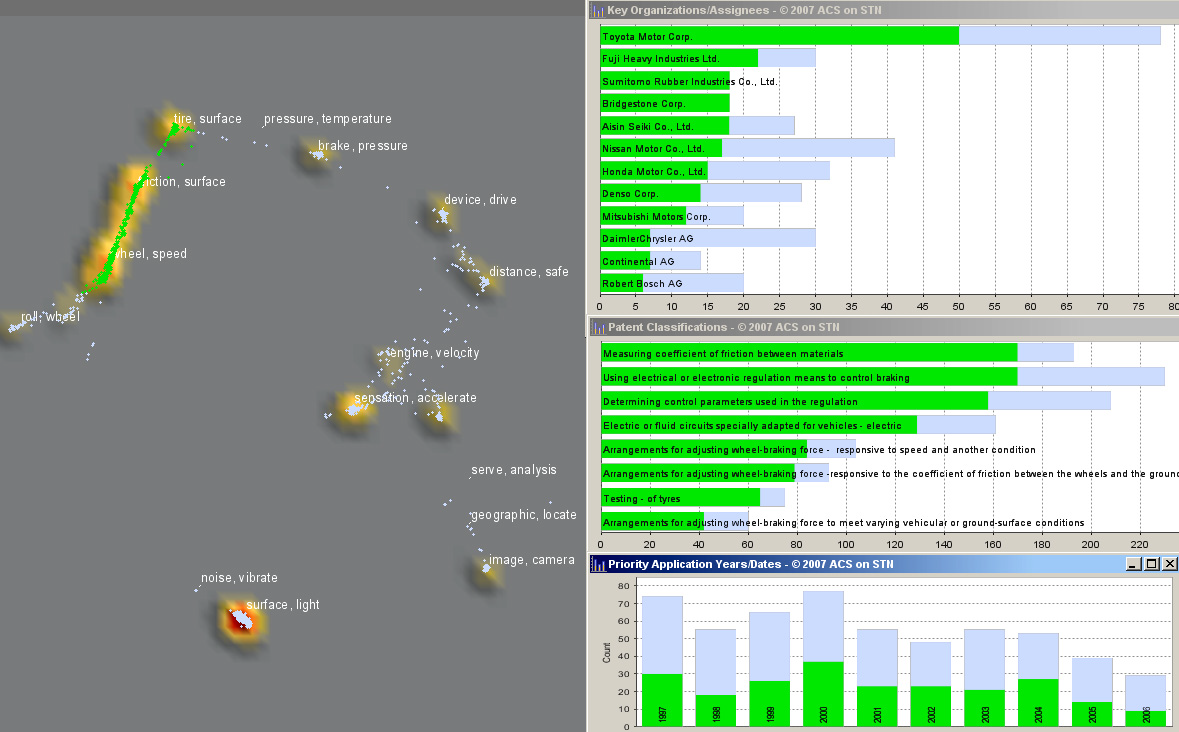
\includegraphics[width=\textwidth]{img/anavist}
\caption{Screenshot of STN AnaVist, a commercial tool for patent landscaping. A selected subset of the data is highlighted in green. Image source: \cite{Ruotsalainen2008}}
\label{fig:anavist}
\end{sidewaysfigure}

\subsection{Summary}

Many approaches use topic modeling as a way to give meaning to the positions in the visualization space.
Others use similarity metrics based on word frequencies to cluster documents.
Only one approach (Federico et al. \cite{Federico2017}) uses semantic word embeddings instead of word-frequency-based features.

Very few works handle patent classification data, which is why we explicitly focus on finding an appropriate visual metaphor for \gls{ipc} classes.

Ultimately, we are unaware of any approach that 1) relies on semantic embeddings to show local and global structures within a dataset, 2) organizes themes into a conceptual hierarchy via clustering and at the same time 3) enables exploration of document metadata through additional visual dimensions or interaction techniques.
This is the research gap we address in this work.